
\begin{figure}[h!]\centering
\captionsetup{width=\textwidth}
\caption{Framework for Calculating the Pumping Cost Externality}
\label{fig:open_access_cartoons}
\vspace{-1mm}
{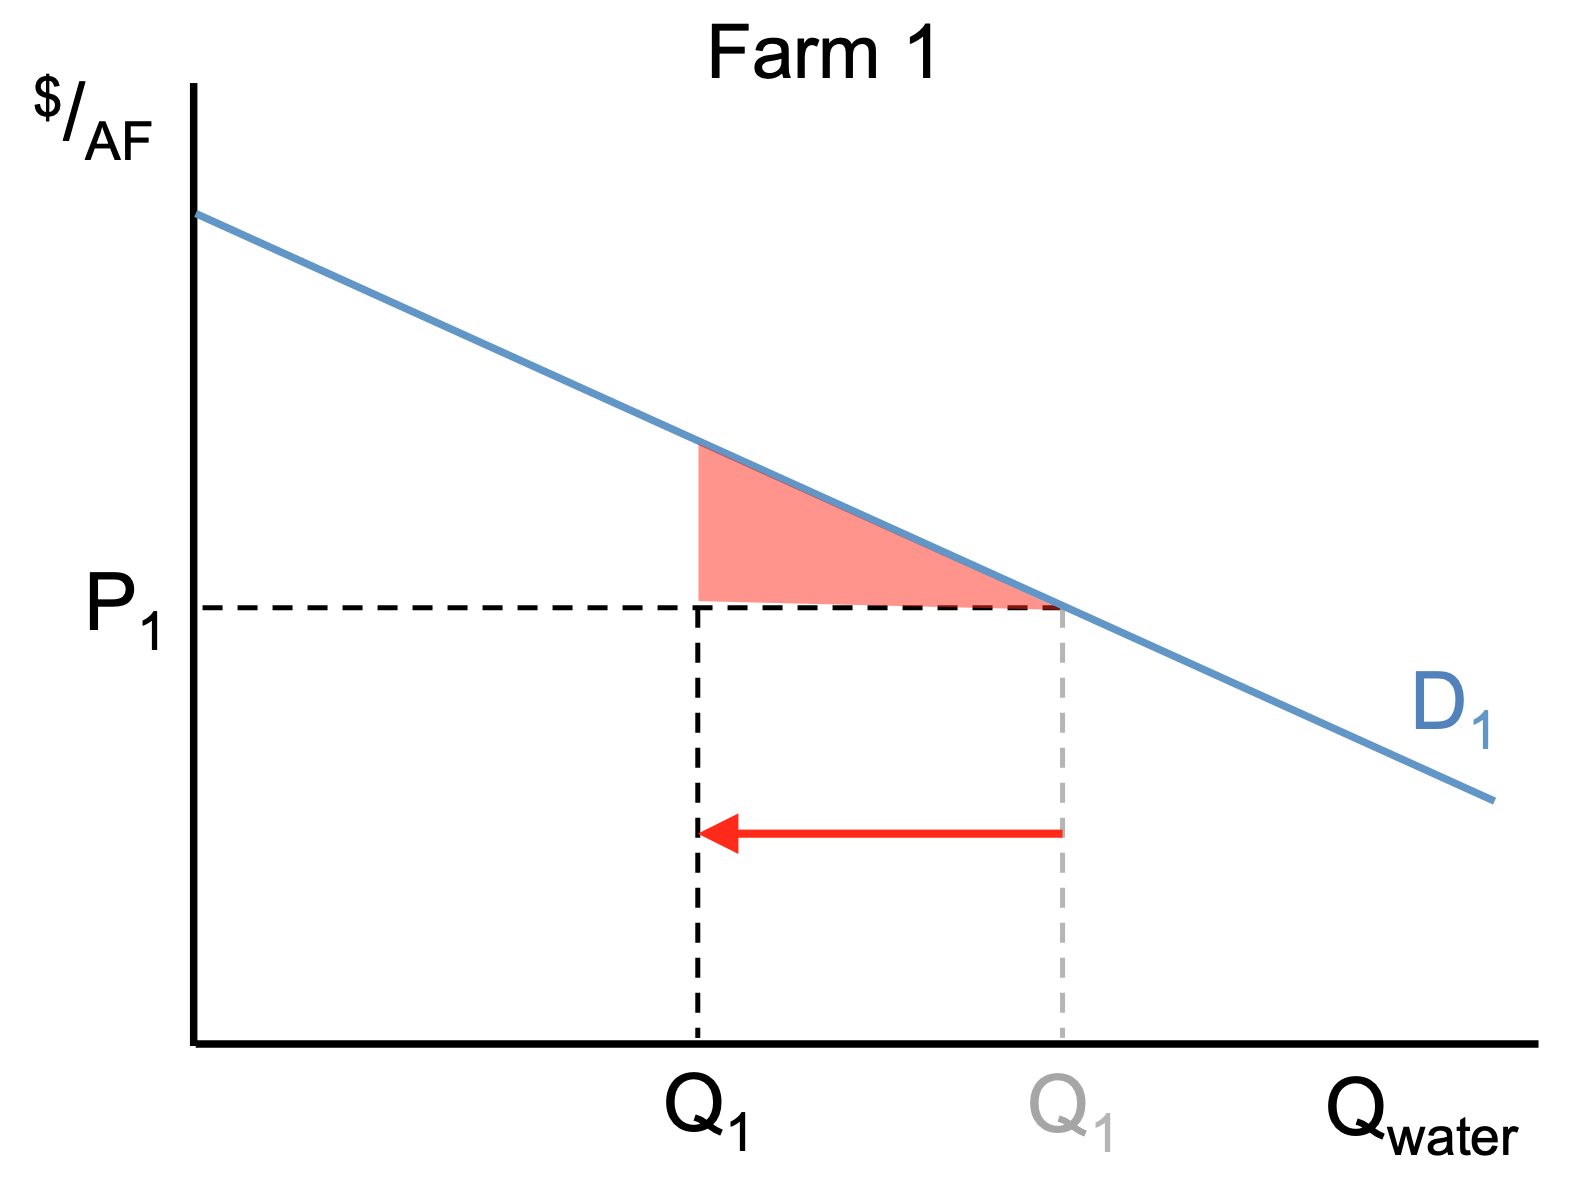
\includegraphics[width=.485\textwidth]{figures/cartoon_1c.png}}~
{\includegraphics[width=.485\textwidth]{figures/cartoon_2c.png}}\\
\vspace{3mm}
{\includegraphics[width=.485\textwidth]{figures/cartoon_3c.png}}~
{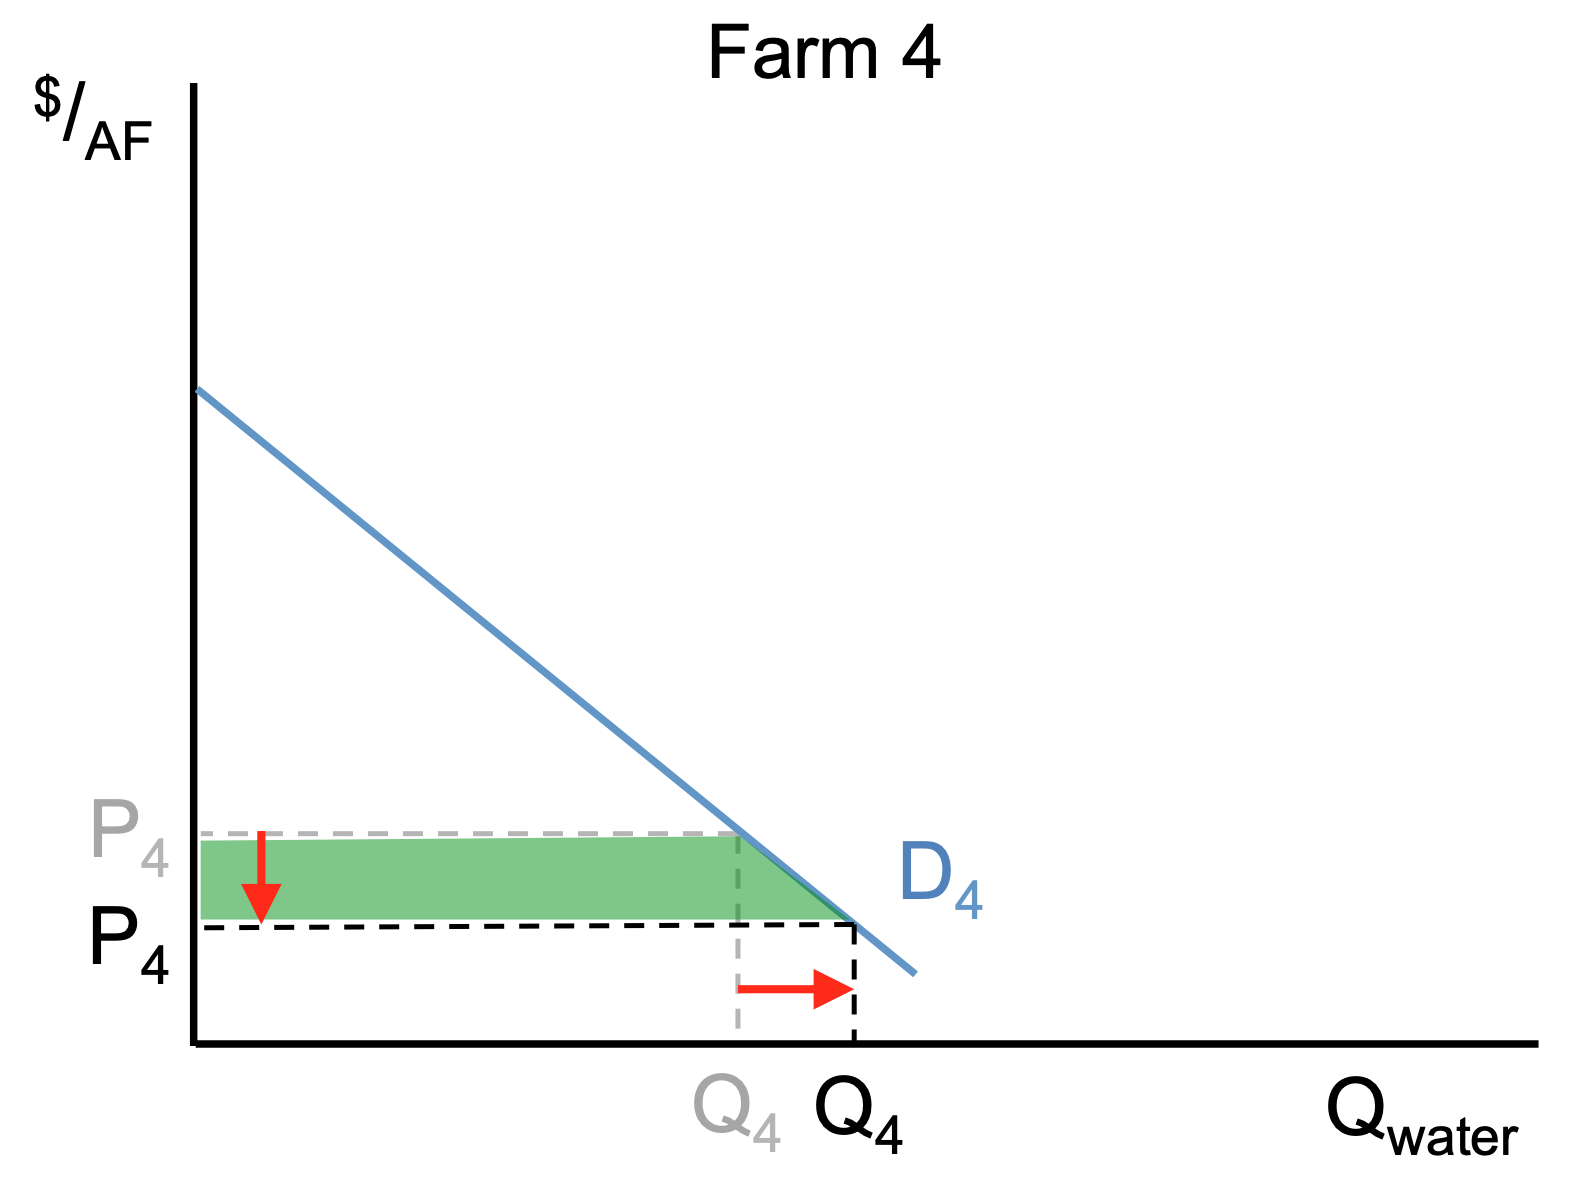
\includegraphics[width=.485\textwidth]{figures/cartoon_4c.png}}\\
\vspace{3mm}
\captionsetup{width=.\textwidth}
\caption*{\footnotesize \emph{Notes:} 
This figure illustrates how we conceptualize and calculate the pumping cost externality that farm $i$ imposes on its neighbors---by not internalizing how its own groundwater extraction increases extraction costs for other nearby farms. In this example, Farm 1 has three neighbors (Farms 2, 3, and 4), and all four farms have distinct demand curves for groundwater. If Farm 1 pumps less than its desired quantity of groundwater, its consumer surplus falls (illustrated by the red triangle). However, when Farm 1 extracts less groundwater, this slightly increases groundwater levels for neighboring Farms 2, 3, and 4. Because Farms 2, 3, and 4 have distinct pumping technologies and electricity prices, a parallel increase in groundwater levels leads to idiosyncratic decreases in their effective prices of groundwater. Farms 2, 3, and 4 respond to these price decreases by slightly increasing groundwater extraction, leading to increased consumer surplus (illustrated by the green trapezoids). If the sum of the (green)  surplus gains for all of Farm 1's neighbors (i.e.\ the pumping cost externality) is greater than Farm 1's own (red) surplus loss, then the Social Planner can increase welfare by taxing Farm 1's groundwater extraction.
 }
\end{figure}